% Nallino, Part II p. 250, note 4: the inclination of the epicycle's diameter seen from the Earth, redrawn from the
% print at the size of the print. The coordinates are those of a 400 dpi render of the figure (crop from x 334 pt,
% y 612 pt of the master page; y downward). AP is the diameter of the epicycle through its centre H, E the Earth;
% the line EH is continued beyond H dashed; the double arc marks the angle of 2 1/2 degrees at H.
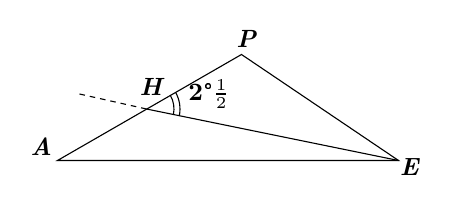
\begin{tikzpicture}[x=0.0635mm,y=-0.0635mm,line width=0.4pt,every node/.style={font=\bfseries\itshape\small,inner sep=1pt}]
\coordinate (A) at (90,313);
\coordinate (P) at (458,101);
\coordinate (E) at (772,313);
\coordinate (H) at (268,210);
\draw (A) -- (P) -- (E) -- cycle;
\draw (H) -- (E);
\draw[dash pattern=on 2pt off 1.8pt] (H) -- (134,180);
\draw (H) ++(-29.8:55) arc[start angle=-29.8, end angle=11.5, radius=55];
\draw (H) ++(-29.8:67) arc[start angle=-29.8, end angle=11.5, radius=67];
\node at (467.5,70) {P};
\node at (276.5,165) {H};
\node[font=\bfseries\small] at (393,180) {2°$\frac{1}{2}$};
\node at (57.5,285) {A};
\node at (793.5,326.5) {E};
\end{tikzpicture}
